\begin{problem}
	Let $\Omega = (-1, +1)^3 \subseteq \R^3$. Let $A, B, C, D, E, F: \Omega \to R$ be sufficiently smooth functions. Let $S = A + B + C + D + E + F$. Consider the 3D equations defined on $\Omega = (-1, +1)^3$
	\begin{align*}
		\frac{\partial A}{\partial x} &= \sigma \tuple*{\frac{1}{6} S - A} \\
		- \frac{\partial B}{\partial x} &= \sigma \tuple*{\frac{1}{6} S - B} \\
		\frac{\partial C}{\partial y} &= \sigma \tuple*{\frac{1}{6} S - C} \\
		- \frac{\partial D}{\partial y} &= \sigma \tuple*{\frac{1}{6} S - D} \\
		\frac{\partial E}{\partial z} &= \sigma \tuple*{\frac{1}{6} S - E} \\
		- \frac{\partial F}{\partial z} &= \sigma \tuple*{\frac{1}{6} S - F}
	\end{align*}
	
	The boundary conditions are 
	\begin{align*}
		A(-1, y, z) &= \phi(y, z) \\
		C(x, -1, z) &= \phi(x, z) \\
		E(x, y, -1) &= \phi(x, y) \\
		B(1, y, z) &= D(x, 1, z) = F(x, y, 1) = 0
	\end{align*}
	
	where $\phi(p, q) = \begin{cases}
		1 &\text{if $|p| \leq 0.2$ and $|q| \leq 0.2$} \\
		0 &\text{otherwise}
	\end{cases}$

	Solve this system of equations numerically for $\sigma = 0.1, 1, 10, 100$. Assume $\sigma = 1/\epsilon$. Consider the time-dependent equations
	\begin{align*}
		\frac{\partial A}{\partial t} + \frac{\partial A}{\partial x} &= \sigma \tuple*{\frac{1}{6} S - A} \\
		\frac{\partial B}{\partial t} - \frac{\partial B}{\partial x} &= \sigma \tuple*{\frac{1}{6} S - B} \\
		\frac{\partial C}{\partial t} + \frac{\partial C}{\partial y} &= \sigma \tuple*{\frac{1}{6} S - C} \\
		\frac{\partial D}{\partial t} - \frac{\partial D}{\partial y} &= \sigma \tuple*{\frac{1}{6} S - D} \\
		\frac{\partial E}{\partial t} + \frac{\partial E}{\partial z} &= \sigma \tuple*{\frac{1}{6} S - E} \\
		\frac{\partial F}{\partial t} - \frac{\partial F}{\partial z} &= \sigma \tuple*{\frac{1}{6} S - F}
	\end{align*}

	Derive the equation of $S$ that approximates the system $A, B, C, D, E, F$ up to the first order
		
\end{problem}

\section{NUMERICAL METHODS}

The numerical method consists of the following steps:
\begin{enumerate}
	\item Discretizing $\Omega$ into grid
	\item Using upwind method to approximate $\frac{\partial U}{\partial w}$ for $U = A, B, C, D, E, F$ and $w = x, y, z$
	\item Decoupling the system of equations
\end{enumerate}

\subsection{DISCRETIZING $\Omega$ INTO GRID}

By symmetry of the equations, we will discretize $\Omega$ into grid of $n \times n \times n$ cells where the distance between centers of two adjacent cells is $h = 2 / n$

\subsection{UPWIND METHOD}

Let $U_{i, j, k}$ denote the value of $A, B, C, D, E, F$ at cell $(i, j, k)$. Since we know the boundary of $A$ at $x = -1$ and $B$ at $x = +1$, we will approximate


\begin{align*}
	\frac{\partial A}{\partial x} &\approx \frac{A_{i, j, k} - A_{i-1, j, k}}{h} \\
	- \frac{\partial B}{\partial x} &\approx \frac{B_{i, j, k} - B_{i+1, j, k}}{h}
\end{align*}

Similarly for $C, D, E, F$, we have

\begin{align*}
	\frac{\partial C}{\partial y} &\approx \frac{C_{i, j, k} - C_{i, j-1, k}}{h} \\
	- \frac{\partial D}{\partial y} &\approx \frac{D_{i, j, k} - D_{i, j+1, k}}{h} \\
	\frac{\partial E}{\partial z} &\approx \frac{E_{i, j, k} - E_{i, j, k-1}}{h} \\
- \frac{\partial F}{\partial z} &\approx \frac{F_{i, j, k} - F_{i, j, k+1}}{h}
\end{align*}


We have the system of equations
\begin{align*}
	\frac{A_{i, j, k} - A_{i-1, j, k}}{h} &= \sigma \tuple*{\frac{1}{6} S_{i, j, k} - A_{i, j, k}} \\
	\frac{B_{i, j, k} - B_{i+1, j, k}}{h} &= \sigma \tuple*{\frac{1}{6} S_{i, j, k} - B_{i, j, k}} \\
	\frac{C_{i, j, k} - C_{i, j-1, k}}{h} &= \sigma \tuple*{\frac{1}{6} S_{i, j, k} - C_{i, j, k}} \\
	\frac{D_{i, j, k} - D_{i, j+1, k}}{h} &= \sigma \tuple*{\frac{1}{6} S_{i, j, k} - D_{i, j, k}} \\
	\frac{E_{i, j, k} - E_{i, j, k-1}}{h} &= \sigma \tuple*{\frac{1}{6} S_{i, j, k} - E_{i, j, k}} \\
	\frac{F_{i, j, k} - F_{i, j, k+1}}{h} &= \sigma \tuple*{\frac{1}{6} S_{i, j, k} - F_{i, j, k}}
\end{align*}

So that we can iteratively calculate the value of $A, C, E$ from small indices to large indices and $B, D, F$ from large indices to small indices

\subsection{DECOUPLING THE SYSTEM OF EQUATIONS}

\subsubsection{EXPLICIT METHOD}

In explicit method, in each iteration, we calculate the right hand side using previous calculated values, at $t$-th iteration, we calculate the next value as follows:
\begin{align*}
	\frac{A_{i, j, k}^{(t)} - A_{i-1, j, k}^{(t)}}{h} &= \sigma \tuple*{\frac{1}{6} S_{i, j, k}^{(t-1)} - A_{i, j, k}^{(t-1)}} \\
	\frac{B_{i, j, k}^{(t)} - B_{i+1, j, k}^{(t)}}{h} &= \sigma \tuple*{\frac{1}{6} S_{i, j, k}^{(t-1)} - B_{i, j, k}^{(t-1)}} \\
	\frac{C_{i, j, k}^{(t)} - C_{i, j-1, k}^{(t)}}{h} &= \sigma \tuple*{\frac{1}{6} S_{i, j, k}^{(t-1)} - C_{i, j, k}^{(t-1)}} \\
	\frac{D_{i, j, k}^{(t)} - D_{i, j+1, k}^{(t)}}{h} &= \sigma \tuple*{\frac{1}{6} S_{i, j, k}^{(t-1)} - D_{i, j, k}^{(t-1)}} \\
	\frac{E_{i, j, k}^{(t)} - E_{i, j, k-1}^{(t)}}{h} &= \sigma \tuple*{\frac{1}{6} S_{i, j, k}^{(t-1)} - E_{i, j, k}^{(t-1)}} \\
	\frac{F_{i, j, k}^{(t)} - F_{i, j, k+1}^{(t)}}{h} &= \sigma \tuple*{\frac{1}{6} S_{i, j, k}^{(t-1)} - F_{i, j, k}^{(t-1)}}
\end{align*}

In particular, $A_{i, j, k}^{(t)} = A_{i-1, j, k}^{(k)} + h \sigma \tuple*{\frac{1}{6} S_{i, j, k}^{(t-1)} - A_{i, j, k}^{(t-1)}}$. Similarly for $B, C, D, E, F$.

\subsubsection{SEMI-IMPLICIT METHOD}

In implicit method, we calculate the right hand side using the current iteration values. However, this at least requires solving a system of $6$ equations. Moreover, since the direction of upwind are different between $A$ and $B$, the number of equations we need to solve is proportional to number of cells. Hence, we use the semi-implicit method as follows: in each iteration of calculating $U$, we will use the current value of $U$ and previous values of all other terms

\begin{align*}
	\frac{A_{i, j, k}^{(t)} - A_{i-1, j, k}^{(t)}}{h} &= \frac{1}{6}\sigma \tuple*{S_{i, j, k}^{(t-1)} - A_{i, j, k}^{(t-1)} - 5 A_{i, j, k}^{(t)}} \\
	\frac{B_{i, j, k}^{(t)} - B_{i+1, j, k}^{(t)}}{h} &= \frac{1}{6}\sigma \tuple*{S_{i, j, k}^{(t-1)} - B_{i, j, k}^{(t-1)} - 5 B_{i, j, k}^{(t)}} \\
	\frac{C_{i, j, k}^{(t)} - C_{i, j-1, k}^{(t)}}{h} &= \frac{1}{6}\sigma \tuple*{S_{i, j, k}^{(t-1)} - C_{i, j, k}^{(t-1)} - 5 C_{i, j, k}^{(t)}} \\
	\frac{D_{i, j, k}^{(t)} - D_{i, j+1, k}^{(t)}}{h} &= \frac{1}{6}\sigma \tuple*{S_{i, j, k}^{(t-1)} - D_{i, j, k}^{(t-1)} - 5 D_{i, j, k}^{(t)}} \\
	\frac{E_{i, j, k}^{(t)} - E_{i, j, k-1}^{(t)}}{h} &= \frac{1}{6}\sigma \tuple*{S_{i, j, k}^{(t-1)} - E_{i, j, k}^{(t-1)} - 5 E_{i, j, k}^{(t)}} \\
	\frac{F_{i, j, k}^{(t)} - F_{i, j, k+1}^{(t)}}{h} &= \frac{1}{6}\sigma \tuple*{S_{i, j, k}^{(t-1)} - F_{i, j, k}^{(t-1)} - 5 F_{i, j, k}^{(t)}}
\end{align*}

In particular,


$$
	A_{i, j, k}^{(t)} = \frac{A_{i-1, j, k}^{(t)} + \frac{1}{6} h\sigma (S_{i, j, k}^{(t-1)} - A_{i, j, k}^{(t-1)})}{\tuple*{1 + \frac{5}{6} h \sigma}}
$$




\section{NUMERICAL SETTINGS}

We divided $\Omega$ into $100 \times 100 \times 100$ grid cells ($n = 100$) and set value of $A, B, C, D, E, F$ into $0$ initially. Then, we update $A, B, C, D, E, F$ iteratively using the previously described method until residue is less than $\epsilon = 1e-6$ where the residue is calculated by

\begin{align*}
	r_{i, j, k} = \tuple*{- \frac{A_{i, j, k}^{(t)} - A_{i-1, j, k}^{(t)}}{h} + \sigma \tuple*{\frac{1}{6} S_{i, j, k}^{(t-1)} - A_{i, j, k}^{(t-1)}}}^2 \\
	+ \tuple*{- \frac{B_{i, j, k}^{(t)} - B_{i+1, j, k}^{(t)}}{h} + \sigma \tuple*{\frac{1}{6} S_{i, j, k}^{(t-1)} - B_{i, j, k}^{(t-1)}}}^2 \\
	+ \tuple*{- \frac{C_{i, j, k}^{(t)} - C_{i, j-1, k}^{(t)}}{h} + \sigma \tuple*{\frac{1}{6} S_{i, j, k}^{(t-1)} - C_{i, j, k}^{(t-1)}}}^2 \\
	+ \tuple*{- \frac{D_{i, j, k}^{(t)} - D_{i, j+1, k}^{(t)}}{h} + \sigma \tuple*{\frac{1}{6} S_{i, j, k}^{(t-1)} - D_{i, j, k}^{(t-1)}}}^2 \\
	+ \tuple*{- \frac{E_{i, j, k}^{(t)} - E_{i, j, k-1}^{(t)}}{h} + \sigma \tuple*{\frac{1}{6} S_{i, j, k}^{(t-1)} - E_{i, j, k}^{(t-1)}}}^2 \\
	+ \tuple*{- \frac{F_{i, j, k}^{(t)} - F_{i, j, k+1}^{(t)}}{h} + \sigma \tuple*{\frac{1}{6} S_{i, j, k}^{(t-1)} - F_{i, j, k}^{(t-1)}}}^2
\end{align*}

and $r = \frac{\sum_{i, j, k} r_{i, j, k}}{6 n^3}$. Informally, $r$ is about the square of the difference between left hand side and right hand side.


\section{NUMERICAL RESULTS}

\subsection{EXPLICIT METHOD}

\subsubsection{$\sigma = 0.1$}

When $\sigma = 0.1$, the explicit method converged, the midplane $x-y$ is shown in the figure below

\begin{figure}[H]
	\caption{explicit method for $\sigma = 0.1$}
	\centering
	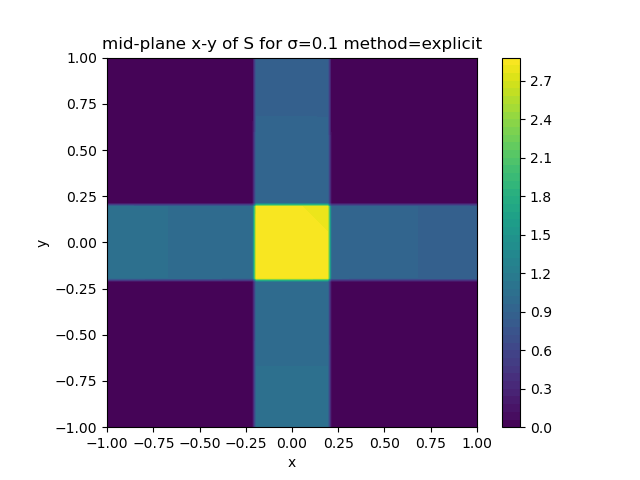
\includegraphics[width=0.7\textwidth]{e_0.1}
\end{figure}

When $\sigma = 1$, the explicit method converged, the midplane $x-y$ is shown in the figure below

\begin{figure}[H]
	\caption{explicit method for $\sigma = 1$}
	\centering
	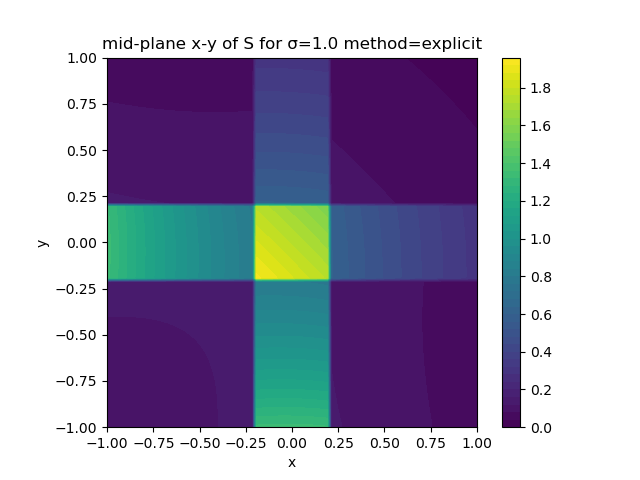
\includegraphics[width=0.7\textwidth]{e_1}
\end{figure}

When $\sigma \geq 10$, the expliciti method failed to converge

\subsection{SEMI-IMPLICIT METHOD}

When $\sigma = 0.1$, the semi-implicit method converged, the midplane $x-y$ is shown in the figure below

\begin{figure}[H]
	\caption{semi-implicit method for $\sigma = 0.1$}
	\centering
	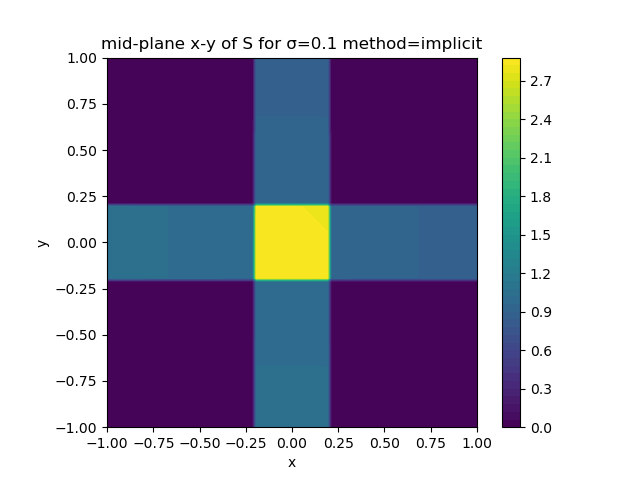
\includegraphics[width=0.7\textwidth]{i_0.1}
\end{figure}

When $\sigma = 1$, the semi-implicit method converged, the midplane $x-y$ is shown in the figure below

\begin{figure}[H]
	\caption{semi-implicit method for $\sigma = 1$}
	\centering
	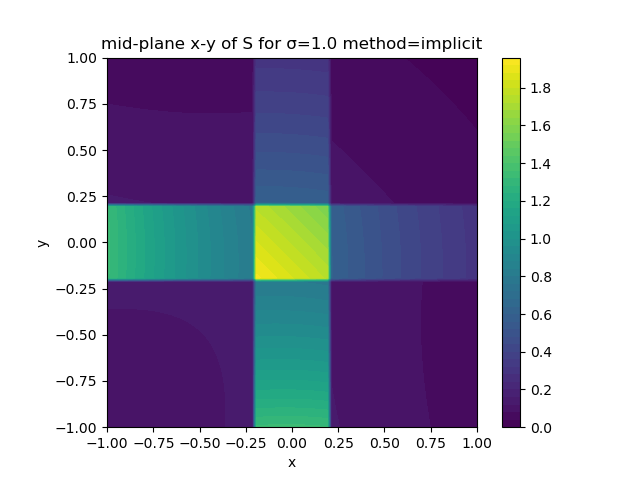
\includegraphics[width=0.7\textwidth]{i_1}
\end{figure}

When $\sigma = 10$, the semi-implicit method converged, the midplane $x-y$ is shown in the figure below

\begin{figure}[H]
	\caption{semi-implicit method for $\sigma = 10$}
	\centering
	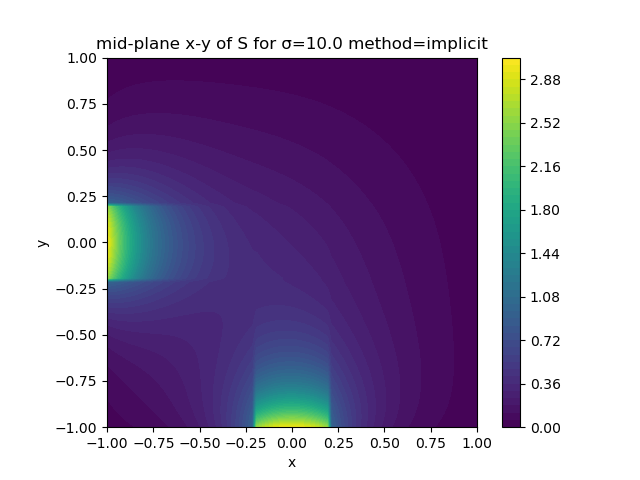
\includegraphics[width=0.7\textwidth]{i_10}
\end{figure}

When $\sigma = 100$, the semi-implicit method converged, the midplane $x-y$ is shown in the figure below

\begin{figure}[H]
	\caption{semi-implicit method for $\sigma = 100$}
	\centering
	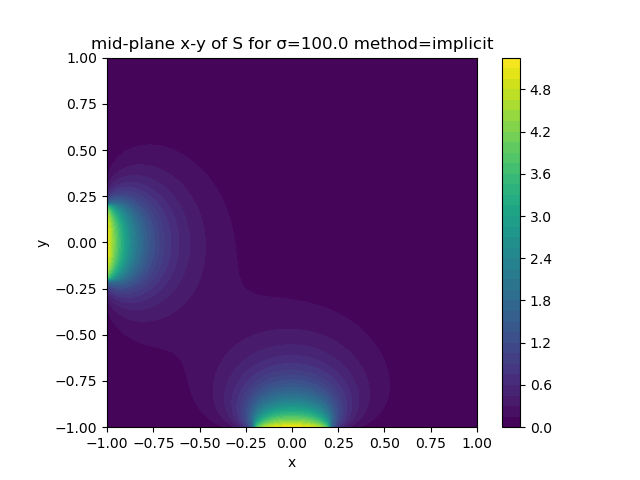
\includegraphics[width=0.7\textwidth]{i_100}
\end{figure}

\subsection{CONVERGENCE OF EXPLICIT METHOD AND SEMI-IMPLICIT METHOD}

\begin{figure}[H]
	\caption{Residue over time for explicit method and semi-implicit method}
	\centering
	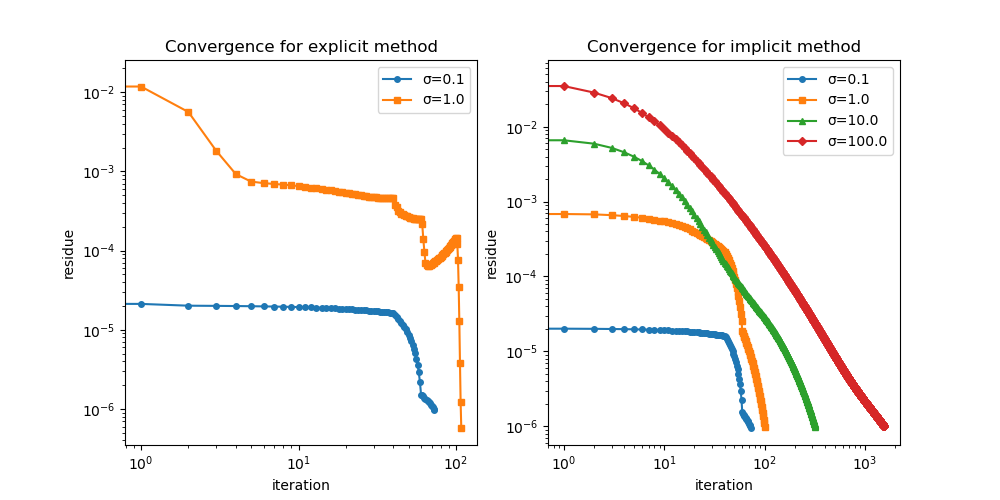
\includegraphics[width=1.0\textwidth]{convergence}
\end{figure}


\section{APPROXIMATE MODEL TO SOLVE FOR $S$}

From the original equation we have

\begin{equation}
	\label{eq_sum}
	\frac{\partial S}{\partial t} + \frac{\partial (A - B)}{\partial x} + \frac{\partial (C - D)}{\partial y} + \frac{\partial (E - F)}{\partial z} = 0
\end{equation}

When $\epsilon \to 0$, suppose the left hand side are of order $O(1)$, we can approximate $A, B, C, D, E, F$ up to the first order as follows:
\begin{align*}
	A &= \frac{1}{6} S + \epsilon A_1 \\
	B &= \frac{1}{6} S + \epsilon B_1 \\
	C &= \frac{1}{6} S + \epsilon C_1 \\
	D &= \frac{1}{6} S + \epsilon D_1 \\
	E &= \frac{1}{6} S + \epsilon E_1 \\
	F &= \frac{1}{6} S + \epsilon F_1
\end{align*}

for some functions $A_1, B_1, C_1, D_1, E_1, F_1: \Omega \times [0, \infty) \to \R$ sufficiently smooth. Then, the equation for $A$ and $B$ become
\begin{align*}
	\tuple*{\frac{1}{6} \frac{\partial S}{\partial t} + \epsilon \frac{\partial A_1}{\partial t}} + \tuple*{\frac{1}{6} \frac{\partial S}{\partial x} + \epsilon \frac{\partial A_1}{\partial x}} = - A_1 \\
	\tuple*{\frac{1}{6} \frac{\partial S}{\partial t} + \epsilon \frac{\partial B_1}{\partial t}} - \tuple*{\frac{1}{6} \frac{\partial S}{\partial x} + \epsilon \frac{\partial B_1}{\partial x}} = - B_1
\end{align*}

At order $O(1)$, we have
\begin{align*}
	A_1 &= - \frac{1}{6}\tuple*{\frac{\partial S}{\partial t} + \frac{\partial S}{\partial x}} \\
	B_1 &= - \frac{1}{6}\tuple*{\frac{\partial S}{\partial t} - \frac{\partial S}{\partial x}} \\
	A - B &= \epsilon(A_1 - B_1) = - \frac{1}{3} \epsilon \frac{\partial S}{\partial x}
\end{align*}

Similar calculation gives
\begin{align*}
	C - D &= - \frac{1}{3} \epsilon \frac{\partial S}{\partial y} \\
	E - F &= - \frac{1}{3} \epsilon \frac{\partial S}{\partial z} 
\end{align*}

Plugging into equation \ref{eq_sum}, we have
$$
	\frac{\partial S}{\partial t} - \frac{1}{3} \epsilon \tuple*{\frac{\partial^2 S}{\partial x^2} + \frac{\partial^2 S}{\partial y^2} + \frac{\partial^2 S}{\partial z^2}} = 0 
$$

which is a diffusion equation with boundary condition.



